\subsubsection{Decimo periodo (2024/05/03 - 2024/05/19)}
\subsubsubsection{Planning}
In questa prima fase, in vista della revisione $\textit{PB}_G$, si è cercato di definire le prime attività, le quali riguardano principalmente la consegna di un $\textit{MVP}_G$. Di conseguenza, molte risorse sono state destinate ai ruoli dei Progettisti e dei Programmatori. \\
A causa dei ritardi considerevoli avuti dal gruppo, si è convenuto, come da suggerimento del prof. Vardanega durante l'ultima parte di revisione $\textit{RTB}_G$, di suddividere, nel corso di una settimana, il gruppo tramite due formazioni composte da tre membri, studiando separatamente le fasi relative alla progettazione e al testing, condividendo a fine della settimana (il 2024/05/10) le informazioni apprese. \\
La seconda parte del periodo, invece, si è concentrata sullo sviluppo dei requisiti necessari per l'$\textit{MVP}_G$ e della messa in pratica del materiale appreso in precedenza, redigendo, parallelamente, il documento di Specifica Tecnica.
\subsubsubsubsection*{Attività pianificate}
Gli obiettivi posti per lo $\textit{sprint}_G$ sono stati i seguenti:
\begin{itemize}
    \item Effettuare degli incontri con il proponente per discutere dei requisti per l'$\textit{MVP}_G$ e dei consigli sull'$\textit{architettura}_G$ da adottare;
    \item Aggiornare il documento di Analisi dei Requisiti;
    \item Aggiornare i documenti, il $\textit{repository}_G$ e il sito web in base alle indicazione fornite in sede di revisione $\textit{RTB}_G$ dal prof. Vardanega:
    \begin{itemize}
        \item Cambiare impostazione dei verbali;
        \item Cambiare impostazione del sito web;
        \item Cambiare impostazione del $\textit{repository}_G$ riservato alla documentazione;
        \item Cambiare impostazione del glossario tecnico;
        \item Modificare $\textit{Norme di Progetto}_G$;
        \item Modificare $\textit{Piano di Qualifica}_G$;
        \item Modificare il presente $\textit{Piano di Progetto}_G$.
    \end{itemize}
    \item Iniziare la stesura del documento di Specifica Tecnica;
    \item Studiare separatamente, tramite una formazione di gruppi composti da tre membri, le fasi relative alla progettazione e al testing, condividendo a fine della settimana (il 2024/05/10) le informazioni apprese. 
    \item Configurare il $\textit{repository}_G$ dedicato all'$\textit{MVP}_G$, inserendo automazioni per effettuare il testing del codice.
    \item Sviluppare alcuni requisiti obbligatori per l'$\textit{MVP}_G$.
\end{itemize}
\subsubsubsubsection*{Preventivo}
\begin{table}[H]
    \centering
\begin{spreadtab}{{tabular}{|c|c|c|c|c|c|c|c|}}
    \hline
    @\textbf{Membro} & @\textbf{Re} & @\textbf{Amm} & @\textbf{An} & @\textbf{Progr} & @\textbf{Proge} & @\textbf{Ve} & @\textbf{Totale} \\
    \hline
    @ Samuele V.   & 2          & 2.67          & 0         & 12.01          & 2.5     & 3.92     & sum(b2:g2) \\
    @ Leonardo B.  & 0         & 1.92          & 0.67        & 0.5        & 0     & 2.17    & sum(b3:g3) \\
    @ Riccardo Z.  & 4.33          & 2.17          & 0          & 5.59         & 4.17     & 1.5 & sum(b4:g4) \\
    @ Davide B.    & 0          & 1.25         & 0.33       & 0       & 0     & 0.17     & sum(b5:g5) \\
    @ Michele Z.   & 0          & 0          & 0         & 0          & 0     & 0.5     & sum(b6:g6) \\
    @ Filippo T.   & 0          & 0          & 0         & 1.33          & 0     & 0.17      & sum(b7:g7) \\
    \hline
    @\textbf{Ore totali} & sum(b2:b7) & sum(c2:c7) & sum(d2:d7) & sum(e2:e7) & sum(f2:f7) & sum(g2:g7) &  sum(b8:g8)\\
    \hline
    @\textbf{Costo totale} & 30*b8 & 20*c8 & 25*d8 & 15*e8 & 25*f8 & 15*g8 & sum(b9:g9)\\
    \hline
\end{spreadtab}
    \caption{Preventivo orario ed economico parziale per il decimo periodo, in base al ruolo}
    \label{tab:prev_rtb}
    \vspace{5mm}
    \textbf{Legenda:} \textit{Re} = Responsabile, \textit{Amm} = Amministratore, \textit{An} = Analista, \textit{Progr} = Programmatore, \textit{Proge} = Progettista, \textit{Ve} = Verificatore
\end{table}
\begin{figure}[H]
    \centering
  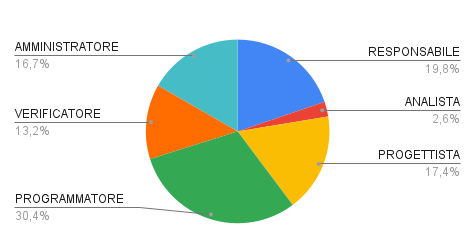
\includegraphics[width=0.6\linewidth]{grafici/10_periodo_torta.png}
  \caption{Preventivo ripartizione dei costi per ruolo nel $10^\circ$ periodo}
        \vspace{5mm}
  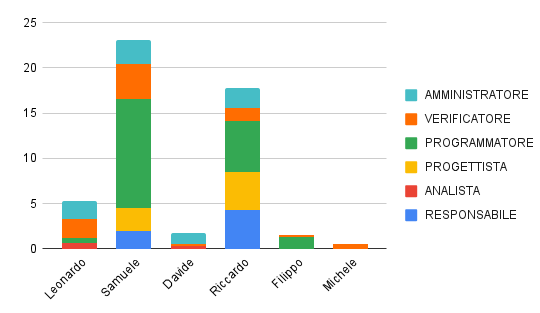
\includegraphics[width=0.7\linewidth]{grafici/10_periodo_istogramma.png}
  \caption{Ore preventivate per ciascuna persona nel $10^\circ$ periodo}
\end{figure}
\subsubsubsection{Review}
Le attività preventivate sono state svolte con successo, risultando un rallentamento solamente per quanto riguarda l'aggiornamento dei documenti secondo le indicazioni fornite in sede di revisione $\textit{RTB}_G$.
\subsubsubsubsection*{Attività svolte}
Le attività svolte in questo periodo sono state le seguenti:
\begin{itemize}
    \item Effettuati tre incontri con il proponente per discutere dei requisiti e dubbi riguardanti la progettazione e la $\textit{codifica}_G$;
\item Aggiornato il documento Analisi dei Requisiti in base a quanto riportato dal proponente relativo all'interazione con lo staff del ristorante tramite chat;
\item Aggiornato il documento $\textit{Norme di Progetto}_G$ con le procedure per la $\textit{codifica}_G$ e la verifica del codice;
\item Aggiornato il documento $\textit{Piano di Qualifica}_G$ con alcune metriche riguardanti la fase di testing;
\item A seguito della valutazione $\textit{RTB}_G$:
\begin{itemize}
    \item Cambiata l'impostazione dei verbali;
    \item Cambiata l'impostazione del sito web;
    \item Cambiata l'impostazione del $\textit{repository}_G$ riservato alla documentazione;
    \item Cambiata l'impostazione del glossario tecnico.
\end{itemize}
\item Completata la progettazione logica e ricevuto $\textit{feedback}_G$ positivo da parte del proponente;
\item Effettuata una prima stesura del documento di Specifica Tecnica;
\item Sviluppati alcuni requisiti funzionali;
\item Implementati i primi $\textit{test}_G$ di unità;
\item Progettato il $\textit{sistema}_G$ di notifica dal punto di vista logico e ricevuto un riscontro positivo da parte del proponente.
\end{itemize}
\subsubsubsubsection*{Consuntivo}
\begin{table}[H]
    \centering
\begin{spreadtab}{{tabular}{|c|c|c|c|c|c|c|c|}}
    \hline
    @\textbf{Membro} & @\textbf{Re} & @\textbf{Amm} & @\textbf{An} & @\textbf{Progr} & @\textbf{Proge} & @\textbf{Ve} & @\textbf{Totale} \\
    \hline
    @ Samuele V.   & 2          & 2.67          & 0        & 15.26        & 2.5     & 3.92    & sum(b2:g2) \\
    @ Leonardo B.  & 0         & 2.17          & 0.67        & 0.5        & 0     & 3.25    & sum(b3:g3) \\
    @ Riccardo Z.  & 4.33         & 1.72          & 0          & 6.75         & 4.17     & 1.92   & sum(b4:g4) \\
    @ Davide B.    & 0          & 1         & 1.5       & 0       & 0     & 1     & sum(b5:g5) \\
    @ Michele Z.   & 0          & 0          & 0         & 1.83          & 0     & 0.17     & sum(b6:g6) \\
    @ Filippo T.   & 0          & 0          & 0         & 0          & 0     & 1     & sum(b7:g7) \\
    \hline
    @\textbf{Ore totali} & sum(b2:b7) & sum(c2:c7) & sum(d2:d7) & sum(e2:e7) & sum(f2:f7) & sum(g2:g7) &  sum(b8:g8)\\
    \hline
    @\textbf{Costo totale} & 30*b8 & 20*c8 & 25*d8 & 15*e8 & 25*f8 & 15*g8 & sum(b9:g9)\\
    \hline
\end{spreadtab}
    \caption{Consuntivo orario ed economico parziale per il decimo periodo, in base al ruolo}
    \label{tab:prev_rtb}
    \vspace{5mm}
    \textbf{Legenda:} \textit{Re} = Responsabile, \textit{Amm} = Amministratore, \textit{An} = Analista, \textit{Progr} = Programmatore, \textit{Proge} = Progettista, \textit{Ve} = Verificatore
\end{table}

\begin{comment}
\begin{figure}[H]
  \centering
  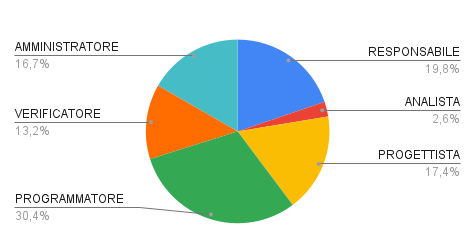
\includegraphics[width=0.6\linewidth]{grafici/10_periodo_torta.png}
  \caption{Ripartizione dei costi per ruolo nel $10^\circ$ periodo}
        \vspace{5mm}
  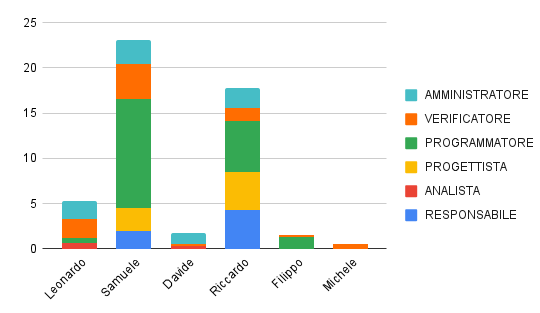
\includegraphics[width=0.7\linewidth]{grafici/10_periodo_istogramma.png}
  \caption{Ore preventivate per ciascuna persona nel $10^\circ$ periodo}
\end{figure}
\end{comment}

\begin{figure}[H]
  \centering
  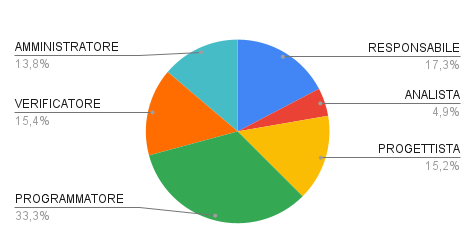
\includegraphics[width=0.6\linewidth]{grafici/10_periodo_torta_consuntivo.png}
  \caption{Consuntivo ripartizione dei costi per ruolo nel $10^\circ$ periodo}
  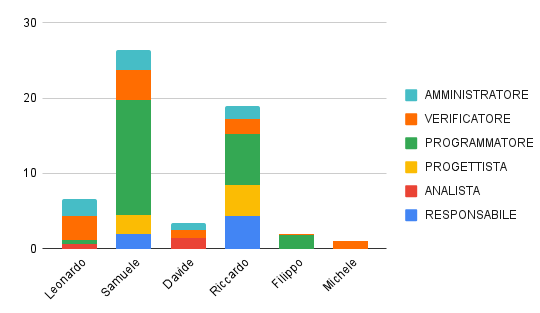
\includegraphics[width=0.7\linewidth]{grafici/10_periodo_instogramma_consuntivo.png}
  \caption{Ore svolte per ciascuna persona nel $10^\circ$ periodo}
\end{figure}

\subsubsubsection{Retrospective}
\paragraph*{Gestione dei Rischi}
I $\textit{rischi}_G$ occorsi per tale periodo sono stati i seguenti:
\begin{itemize}
    \item \nameref{ro:1}: la scarsa esperienza nell'organizzazione di un progetto complesso ha causato un rallentamento previsto nel corso dello $\textit{sprint}_G$. In particolare si è rilevata una sottostima nelle attività di verifica e di programmazione.
    \begin{itemize}
        \item \textbf{Esito mitigazione}: il continuo colloquio tra il responsabile e i membri del gruppo hanno fatto sì di poter estendere la durata delle attività segnalate in modo ragionevole.
        \item \textbf{Impatto}: sono state spese risorse significative non previste andando ad impattare sul modo di calcolare le ore per il progettista e per il verificatore per quanto riguarda la $\textit{codifica}_G$.
    \end{itemize}
    \item \nameref{ro:3}: un membro del gruppo, a causa di impegni lavorativi, non ha potuto eseguire le task assegnatoli.
    \begin{itemize}
        \item \textbf{Esito mitigazione}: le task assegnate al membro del gruppo sono state scelte tra le meno urgenti e "bloccanti" rispetto al resto del progetto non causando rallentamenti significativi.
        \item \textbf{Impatto}: la poca partecipazione nelle attività principali potrebbe causare un rallentamento ulteriore nello studio delle $\textit{tecnologie}_G$ e della progettazione. Al momento non si registrano conseguenze considerevoli. 
    \end{itemize}
    \item \nameref{ro:4}: la scarsa chiarezza nella gestione dei ruoli e delle attività ha causato un rallentamento previsto nel corso dello $\textit{sprint}_G$.
    \begin{itemize}
        \item \textbf{Esito mitigazione}: le attività di studio individuale e di gruppo avevano lo scopo di apprendere come maggiore efficienza i compiti di progettazione e di testing oltre che di chiarire maggiormente i ruoli del progettista e dell'amministratore, tuttavia tutto ciò è risultato per alcuni membri del gruppo in poca chiarezza per quanto riguarda le attività individuali e per la gestione dei ruoli. 
        \item \textbf{Impatto}: alcuni membri del gruppo avevano compreso poco il ruolo assegnatoli rispetto ad altri. Il fatto che alcuni membri del gruppo fossero "più' attivi" ha causato un eccessivo rilassamento in merito allo studio individuale che è andato ad impattare sulla stesura del documento di Specifica Tecnica e lo sviluppo dei $\textit{test}_G$ di unità oltre che sulle attività inerenti future.
    \end{itemize}
    \item \nameref{ro:5}: la scarsa esperienza nella progettazione e nel testing ha causato un rallentamento previsto nel corso dello $\textit{sprint}_G$.
    \begin{itemize}
        \item \textbf{Esito mitigazione}: le attività di studio individuale e il confronto di gruppo e gli incontri frequenti con il proponente sono stati gli elementi principali per mitigare tale rischio. In particolare per ogni risultato ottenuto in fase di testing e di progettazione, si è data una dimostrazione al proponente, ottenendone un riscontro tempestivo. I risultati sono stati soddisfacenti e in linea con quanto preventivato.
        \item \textbf{Impatto}: dopo un primo periodo di incertezza, i membri del gruppo hanno dimostrato di aver appreso maggiormente nell'ambito del testing, meno nell'ambito della progettazione. Nonostante questo, non si sono registrate conseguenze significative.
    \end{itemize}
\end{itemize}
\paragraph*{Considerazioni e pianificazione futura}
\begin{itemize}
    \item Sebbene la progettazione logica sia stata compresa, come dimostra il $\textit{feedback}_G$ positivo da parte del proponente, quella di $\textit{sistema}_G$ presenta alcune parti incomprese relative alle definizione dei $\textit{design}_G$ pattern architetturali e la formazione dei primi diagrammi $\textit{UML}_G$. In futuro, tramite un incontro con il prof. Cardin, si dovrà intervenire su questi dubbi.
    \item Alcuni membri del gruppo, spinti da esigenze personali, sono risultati maggiormente motivati a svolgere le attività assegnateli rispetto ad altri. In particolare, si registra uno sbilanciamento delle ore considerevole tra alcuni di essi. Inoltre, il monte ore raggiunto fino a questo momento non permette di far arrivare alla conclusione tutti i membri del gruppo in un tempo ragionevole. In futuro, bisognerà esplicitare, da parte del responsabile, l'esigenza di svolgere le attività in tempo utile in modo soddisfare le esigenze di tutti i membri e del progetto. 
\end{itemize}
 